\documentclass[xcolor=dvipsnames, USenglish]{beamer}  %notes=show to print them in the generated pdf
% Packages for a reasonable beamer session
\usepackage[T1]{fontenc}
\usepackage[ansinew]{inputenc}
\usepackage{textcomp}
\usepackage{lmodern}
\usepackage{csquotes}
\usepackage{babel}

\usepackage{graphicx}

\usepackage{amsmath}
\usepackage{amsfonts}
\usepackage{amssymb}
\usepackage{amsthm}
\usepackage{bm}

\usepackage{booktabs}
\usepackage{tabularx}

\usepackage{hyperref}

\usepackage{ellipsis}

% Additional packages
\usepackage{graphicx}
\usepackage{subfigure}
\usepackage{xcolor}


\usepackage[style=authoryear, backend=biber]{biblatex}
\setbeamertemplate{itemize/enumerate body begin}{\setlength{\leftmargini}{1.5em}}
\renewcommand*{\nameyeardelim}{\addcomma\addspace}
\addbibresource{\jobname.bib}
\renewcommand{\footnotesize}{\tiny}

\usepackage{tikz,pgf,calc}
%\usetikzlibrary{matrix, shapes, positioning, calc,
%  decorations.pathreplacing, shapes.geometric, arrows}
\usetikzlibrary{shapes.geometric, arrows, calc}
\tikzstyle{startstop} = [rectangle, rounded corners, minimum width=3cm, minimum height=1cm, text centered, text width=1.5cm, draw=black, fill=red!30]
\tikzstyle{io} = [trapezium, trapezium left angle=70, trapezium right angle=110, minimum width=3cm, minimum height=1cm, text centered, draw=black, fill=blue!30]
\tikzstyle{process} = [rectangle, minimum width=3cm, minimum height=1cm, text centered, draw=black, fill=orange!30]
\tikzstyle{decision} = [diamond, minimum width=3cm, minimum height=0.5cm, text centered, draw=black, fill=green!30]
\tikzstyle{arrow} = [thick,->,>=stealth]

%% References
\newlength\leftsidebar
\makeatletter
\setlength\leftsidebar{\beamer@leftsidebar}
\makeatother

\usepackage[absolute,overlay]{textpos}
\newenvironment{reference}[2]{%
  \begin{textblock*}{\textwidth}(\leftsidebar+#1,\paperheight-#2)
      \scriptsize\bgroup\color{red!50!black}}{\egroup\end{textblock*}}

% Path to graphics
\graphicspath{{../img/}}

% Sources
\usepackage{setspace}
\newcommand{\source}[1]{\begin{spacing}{0.5}{\fontsize{5}{6}\selectfont source: \itshape {#1}}\end{spacing}}
 % PACKAGES
% Collection of useful mathematical symbols and commands
% Calculus
\newcommand{\ud}{\mathrm{d}}
\newcommand{\pder}[2]{\frac{\partial{#1}}{\partial{#2}}}
\newcommand{\dpder}[2]{\frac{\partial^2{#1}}{\partial{#2^2}}}
\newcommand{\sderp}[3]{\frac{\partial^2{#1}}{\partial{#2}\partial{#3}}}
\newcommand{\tder}[2]{\frac{\ud{#1}}{\ud{#2}}}
\newcommand{\rot}[1]{\nabla \times {#1}}
\newcommand{\diver}[1]{\nabla \cdot {#1}}
\newcommand{\definter}[4]{\int_{#1}^{#2} {#3}\ud {#4}}
\newcommand{\inter}[2]{\int {#1}\ud {#2}}
\newcommand{\braket}[2]{\langle {#1} , {#2} \rangle}
% Misc
\newcommand{\eval}[1]{\Big |_{#1}}
\newcommand{\bset}[1]{\big\lbrace {#1} \big\rbrace}
\newcommand{\stimes}[2]{{#1}\!\times\!{#2}}
\newcommand{\trp}{\top}
\newcommand{\preup}[2]{{}^{#2}\!{#1}}

% Operators
\DeclareMathOperator*{\armin}{arg\,min}
\DeclareMathOperator*{\armax}{arg\,max}
\DeclareMathOperator*{\rank}{rank}
\DeclareMathOperator*{\cov}{cov}
\DeclareMathOperator*{\nullsp}{null}
% Logicals
\newcommand{\suchthat}{\big \backslash \;}
   % SYMBOLS

% ----------- extra packages
\usepackage{../beamer_themes/beamerthemeEawag_blue} % Eawag style

% ----------- Extra symbols
\newcommand{\ccov}[1]{{\color{red}k}\left(#1\right)}
\newcommand{\cmean}[1]{{\color{blue}m}\left(#1\right)}
\newcommand{\sm}{\scalebox{0.5}{-1}}

% ----------- For boxed equations
\usepackage{amsmath}
\usepackage{empheq}
\usepackage[most]{tcolorbox}
\newtcbox{\mymath}[1][]{%
    nobeforeafter, math upper, tcbox raise base,
    enhanced, colframe=blue!30!black,
    colback=blue!30, boxrule=1pt,
    #1}



%----------------
% title information
\title{A prelude to emulation for \emph{flood prediction}}
\author[\texttt{sebastiano.rusca@eawag.ch}]{Sebastiano Rusca}
\institute[Eawag]{Eawag: Swiss Federal Institute of Aquatic Science
  and Technology}
\date[12.03.2018]{March 12, 2018}
% Title suggestions
% * use an active title: with a verb, or using "in", not "application of ... to ..."
% * not a too bombastic one, "Emulation in hydrology" is too much
% * try to use "shallow water equation", this is what we actually emulate
% * first steps towards ...
% * a guide to emulation in ...


% ====================================================================

\begin{document}

%%%%%%%%%%%%%%%%%%%%%%%%%%%%%%%%%%%%%%%%%%%%%%%%%%%%%%%%%%%%%%%%%%%%%%%%%%%%%%%%

% ----------------
% Title frame
% load background for title
\setbeamertemplate{background}{
  \includegraphics[width=\paperwidth,height=\paperheight]
  {../beamer_themes/background_title_blue_eth.png}}
{ \setbeamertemplate{footline}{} % no footer on title
  \begin{frame}
    \titlepage
  \end{frame}
}
% load background for all other slides
\setbeamertemplate{background}{
\includegraphics[width=\paperwidth,height=\paperheight]
{../beamer_themes/background_slides_blue.png}}
\setbeamertemplate{footline}[Sebastiano Rusca] % set footer
\addtocounter{framenumber}{-1}  % don't count title page

%%%%%%%%%%%%%%%%%%%%%%%%%%%%%%%%%%%%%%%%%%%%%%%
%----------------
\section{Introduction}

  \begin{frame}
    \frametitle{Outline}
    \begin{itemize}
      \item Master thesis goals
      \item What is emulation?
      \item Case studies
      \begin{itemize}
      %\itemsep0em
        \item A mechanistic emulator: \emph{fitting the weir equation}
        \item A hydrological emulator: \emph{estimating the time-to-threshold}
      \end{itemize}
      \item Conclusion
      \item Outlook
     \end{itemize}
  \end{frame}


%%%%%%%%%%%%%%%%%%%%%%%%%%%%%%%%%%%%%%%%%%%%%%%%%%%%%%%%%%%%%%%%%%%%%%%%%%%%%%%%
% MASTER THESIS GOALS
  \begin{frame}
    \frametitle{Master thesis goals}
    \begin{itemize}
      \item Get an overview of emulation
      \begin{itemize}
        \item Learn about \emph{interpolation}, \emph{intrapolation} and \emph{extrapolation}
        \item Learn about \emph{Gaussian Processes}
      \end{itemize}
      \item Find an appropriate \emph{open source} hydrological simulator
      \begin{itemize}
      %\itemsep0em
        \item Learn its \emph{functioning} and \emph{customize} it for the required scope
        \item Produce \emph{datasets} usable for emulation
      \end{itemize}
      \item Perform emulation with a \emph{didactic} example
      \begin{itemize}
      %\itemsep0em
        \item Mechanistic emulator: \emph{the weir equation}
      \end{itemize}
      \item Perform emulation in a \emph{hydrological} context
      \begin{itemize}
      %\itemsep0em
        \item Hydrological emulator: \emph{time-to-threshold}
      \end{itemize}
      \item Draw conclusions about emulation potential, especially applied to the \emph{hydrology},
            \emph{urban water} and \emph{water management} fields
    \end{itemize}
  \end{frame}


%%%%%%%%%%%%%%%%%%%%%%%%%%%%%%%%%%%%%%%%%%%%%%%%%%%%%%%%%%%%%%%%%%%%%%%%%%%%%%%%
% WHAT IS EMULATION?
  \begin{frame}
    \frametitle{What is emulation?}
    bla bla
  \end{frame}


%%%%%%%%%%%%%%%%%%%%%%%%%%%%%%%%%%%%%%%%%%%%%%%%%%%%%%%%%%%%%%%%%%%%%%%%%%%%%%%%
% GAUSSIAN PROCESSES, MACHINE LEARNING
  \begin{frame}
    \frametitle{Machine learning techniques}
    bla bla
  \end{frame}


%%%%%%%%%%%%%%%%%%%%%%%%%%%%%%%%%%%%%%%%%%%%%%%%%%%%%%%%%%%%%%%%%%%%%%%%%%%%%%%%
% CASE STUDIES
  {
  \setbeamertemplate{background}{}
  \setbeamercolor{background canvas}{bg=black}
  \setbeamercolor{normal text}{fg=white}
  \usebeamercolor[fg]{normal text}
  \begin{frame}[plain]
    \centering
    \Large{\textbf{Case studies}}\\
  \end{frame}
  }


%%%%%%%%%%%%%%%%%%%%%%%%%%%%%%%%%%%%%%%%%%%%%%%%%%%%%%%%%%%%%%%%%%%%%%%%%%%%%%%%
% CASE STUDY 1: OVERVIEW
\section{Case study 1: weir equation}

  \begin{frame}
    \frametitle{Mechanistic emulator: \emph{the weir equation}}
    \textbf{Goal}: fit the weir equation to simulated data\\
    \vfill
    \begin{alertblock}{Weir equation}
      \setlength\abovedisplayskip{0pt}
      \begin{equation*}
        Q = \frac{2}{3}\: \textcolor{red}{\mu}\: B_w\: \sqrt{2g}\: h_w^{\textcolor{red}{a}},
        \quad usu.\: \textcolor{red}{a = 3/2}
      \end{equation*}
    \end{alertblock}
    \vfill
    \centering
    $\boldsymbol{\mu :\,}$ \raisebox{-.2\height}{\includegraphics[width=0.8\textwidth]{img/weir_coefficients.png}}
    \source{Boes, Robert. "Wasserbau - Vorlesungsmanuskript." ETH Z\"urich - VAW, 2016.}
  \end{frame}
% * In this first case study we want to fit the weir equation to simulated data.
% * In a while we will see what relation this has with emulation and machine learning.
% * The weir equation can be derived analytically by assuming no friction losses and 
%   a uniform velocity distribution.
% * Results obtained are for a theoretical discharge, which diverges from empirical results, where
%   the assumption mentioned don't hold.
% * In order to obtain actual discharge a correction factor \mu has to be taken into account.
% * \mu is dependent on the type and shape of weir (broad-crested/narrow-crested) and which
%   particular shape.
% * To obtain the value of this coefficient the equation has to be fitted to 
%   experimental data.
% * Here below some \mu-values for some weir types are shown


%%%%%%%%%%%%%%%%%%%%%%%%%%%%%%%%%%%%%%%%%%%%%%%%%%%%%%%%%%%%%%%%%%%%%%%%%%%%%%%%
% CASE STUDY 1: STUDY SET-UP
  \begin{frame}
    \frametitle{Simulations set-up}
    \textbf{Input discharge}
    \inputminted[fontsize=\scriptsize,
                firstline=1,
                lastline=2,
                numbersep=2pt,
                gobble=0,
                frame=lines,
                bgcolor=bg,
                framesep=2mm]{octave}
                {code.m}
    \vfill
    \textbf{Channel set-up}

    \centering
    \includegraphics[width=0.8\textwidth]{img/weir.png}
  \end{frame}
% * Mention FullSWOF_2D


%%%%%%%%%%%%%%%%%%%%%%%%%%%%%%%%%%%%%%%%%%%%%%%%%%%%%%%%%%%%%%%%%%%%%%%%%%%%%%%%
% CASE STUDY 1: SIMULATIONS RESULTS
  \begin{frame}
    \frametitle{Simulations results}
    \begin{minipage}{.5\textwidth}
      \centering
      \small{Experiments free-surfaces}\\
      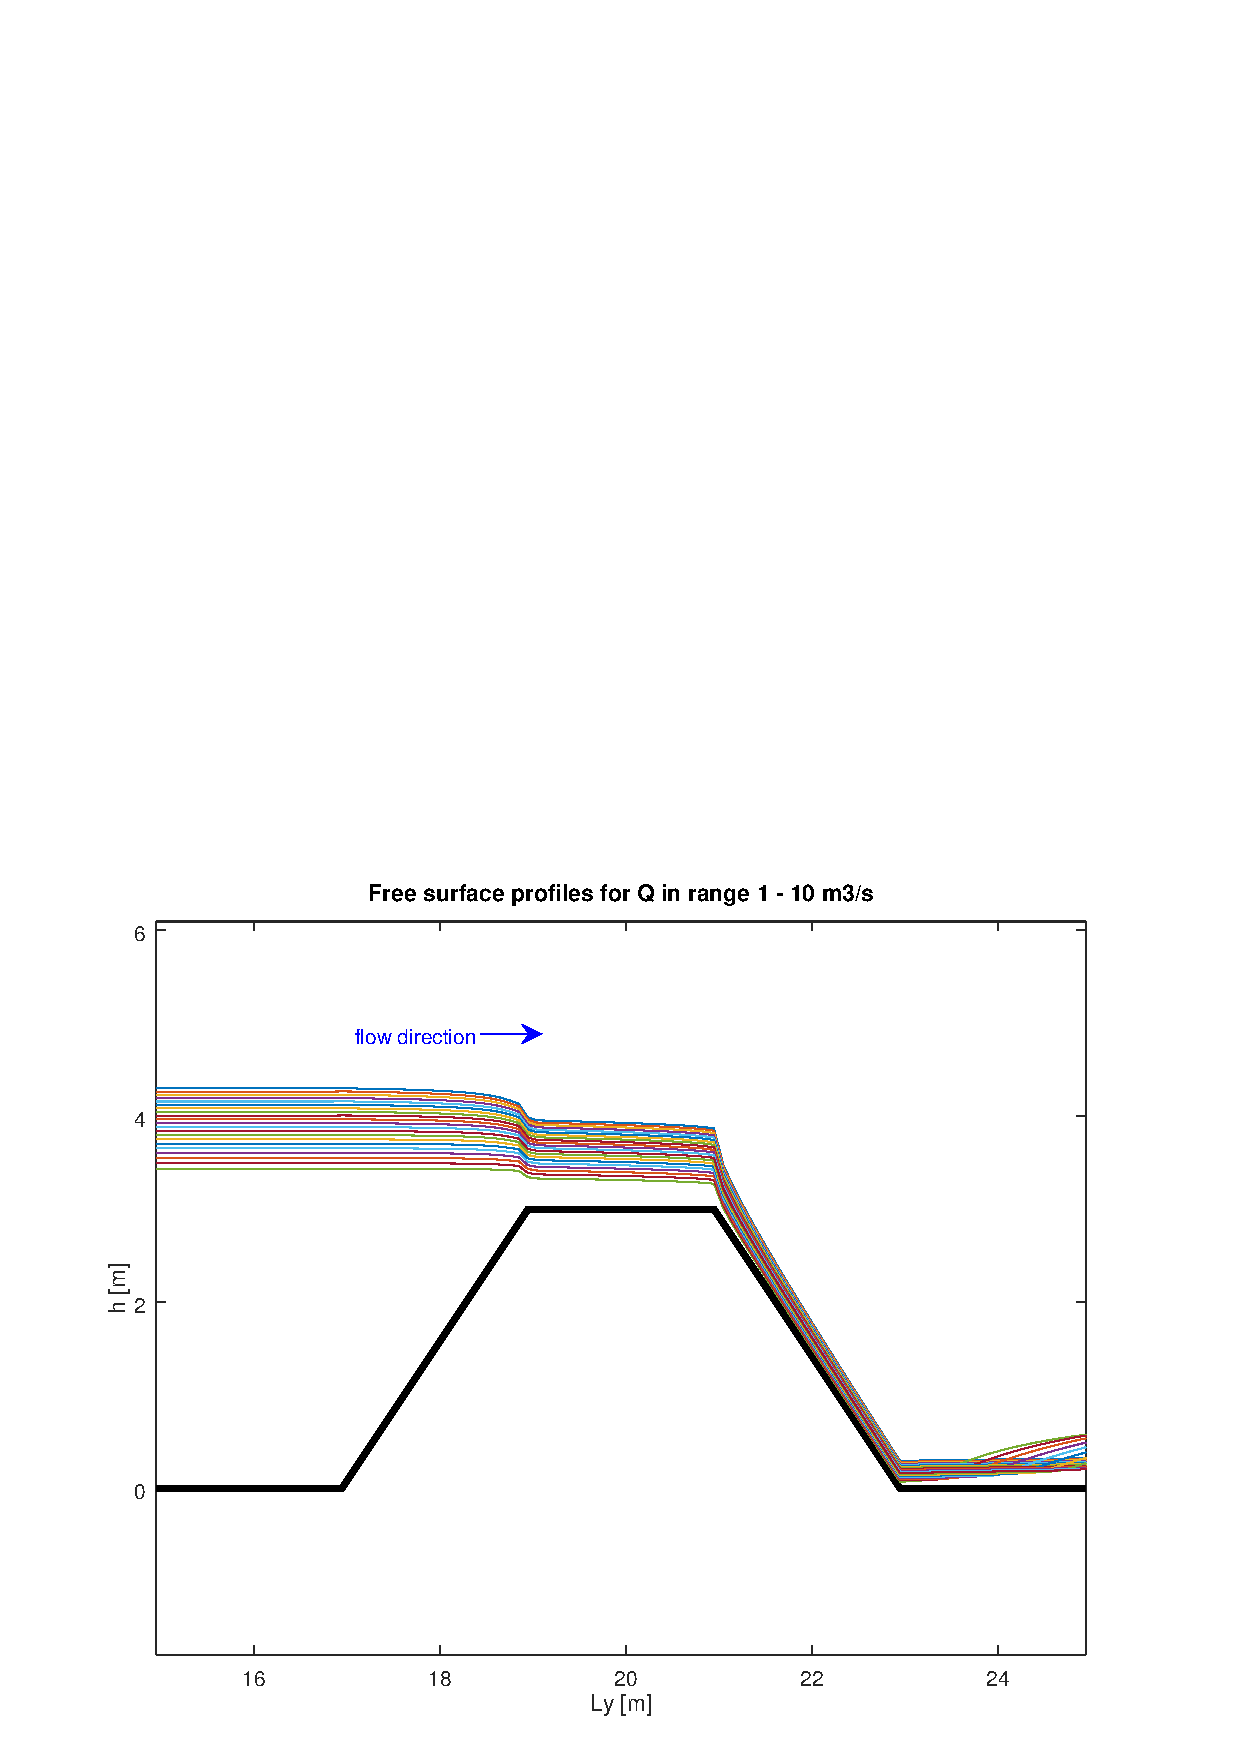
\includegraphics[width=\textwidth]{img/free_surfaces.png}
    \end{minipage}%
    \begin{minipage}{.5\textwidth}
      \centering
      \small{Experiments $h_w$ vs. $Q$}\\
      \includegraphics[width=\textwidth]{img/simulation_results.png}
    \end{minipage}
  \end{frame}


%%%%%%%%%%%%%%%%%%%%%%%%%%%%%%%%%%%%%%%%%%%%%%%%%%%%%%%%%%%%%%%%%%%%%%%%%%%%%%%%
% CASE STUDY 1: FITTING RESULTS
  \begin{frame}
    \frametitle{Fitting results}
    \begin{minipage}{.5\textwidth}
      \centering
      \small{Fitting different models}\\
      \includegraphics[width=\textwidth]{img/fitting_results.png}
    \end{minipage}%
    \begin{minipage}{.5\textwidth}
      \centering
      \small{Fitting performance}\\
      \includegraphics[width=\textwidth]{img/fitting_errors.png}
    \end{minipage}
    \vfill
    \pause
    \small{\textbf{Take home message}: if we have the right model we do not need much data to perform a good fitting}
  \end{frame}
% * 3 different fittings were done
% * Weir equation follows a power law, therefore the logarithm of the data was taken
%   and a linear regression was performed with all data.
%   values of \mu = 0.56 and a = 1.59 were found.
% * A linear interpolation was performed. performs very bad at the beginning (few points),
%   but quite good afterwards (almost overlaying).
% * A spline interpolation was performed. This performs good even between points
%   1 and 2 (almost overlaying).
% * I wanted to test the robustness of the different methods
% * I took a subset of the training dataset (14 points, otherwise computation too long) and
%   performed cross-validation leaving out 1, 2, ... up to 10 points.
% * Every time all possible combination of left-out points were tested and the
%   mean squared error was computed.
% * The plot shows the mean of the mean squared errors of all possible subsets by
%   leaving out 1, 2, ... 10 points.
% * When 10 points were left out just 4 were used for training: 1st, last + 2 random points.
% * From the plot we see some interesting features:
% * The  linear fit always performs the worst, although not even that bad: RMSE of ~2cm
%   leaving out 1 point.
% * The spline fit performs very good, better than the weir equation model thanks to its
% * very high flexibility. However, its error increases very rapidly by reducing
%   the number of training points. There is no prior knowledge encoded in the spline model,
%   it is just a fit to the data. When there are few training points the spline can move
%   very freely in between, and get far from the points generated by the process.
% * With 9 and 10 points left out the spline model performs worse than the weir equation model.
% * The weir equation encodes prior knowledge: the physics of the process.
% * The error here grows very slowly, the model performs very well even if trained on 4 points, 
%   and here actually better than the spline model.
% * Take home message: if we have knowledge about the process we don't need data


%%%%%%%%%%%%%%%%%%%%%%%%%%%%%%%%%%%%%%%%%%%%%%%%%%%%%%%%%%%%%%%%%%%%%%%%%%%%%%%%
% CASE STUDY 2: OVERVIEW
\section{Case study 2: time-to-threshold}

  \begin{frame}
    \frametitle{Hydrological emulator: \emph{time-to-threshold}}
    \textbf{Goal}: build an emulator to estimate the \emph{time-to-threshold}\\
    \vfill
    \centering
    \includegraphics[width=0.6\textwidth]{img/flood_bridge.jpg}
    \source{https://www.dailyrecord.co.uk/news/scottish-news/storm-frank-rescuers-brave-storm-7096067}
  \end{frame}
% * Building an emulator to estimate the time to threshold:
%   Our hydraulic structures (bridges, embankments, ...) have thresholds for which they were
%   sized. If those thresholds are exceeded, then the structure cannot fulfill its function.
% * Measures have to be taken in this case, build up temporary flood-blocking barriers,
%   evacuate people, etc.
% * We want to build up an emulator able, for a given catchment, knowing the rain intensity
%   over the catchment and the initial moisture content of its soil, to estimate after how long
%   the threshold discharge value at its outlet will be exceeded.
% * Such an emulator could for example be used as an early flood warning system

%%%%%%%%%%%%%%%%%%%%%%%%%%%%%%%%%%%%%%%%%%%%%%%%%%%%%%%%%%%%%%%%%%%%%%%%%%%%%%%%
% CASE STUDY 2: STUDY SET-UP
  \begin{frame}
    \frametitle{Simulation set-up}
    \centering
    \includegraphics[width=0.7\textwidth]{img/topography.png}
    \inputminted[fontsize=\scriptsize,
                firstline=6,
                lastline=9,
                numbersep=2pt,
                gobble=0,
                frame=lines,
                bgcolor=bg,
                framesep=2mm]{octave}
                {code.m}
  \end{frame}
% * For this case study the synthetic topography that you see here was created using
%   the open source tool "GNU Octave"
% * This represents a catchment of 2 km x 2 km and is composed of three "Gaussian bumps"
%   on a sloping plane. The three Gaussian bumps generate a Y-shaped channel which goes
%   from the top of the catchment up to the bottom.
% * The synthetic topography presents a surface which is very smooth. This way a coarse
%   grid resolution can be used, without having loss of important features.
% * As for the first case study, the simulator "FullSWOF_2D" was used for running the simulations.
% * 50 different rain events were simulated on this topography.
% * Every simulated rain event is distinguished by a different combination of the parameters
%   initial soil moisture content and rain intensity. 
% * All of the other simulation parameters were kept the same.
% * A linearly spaced grid was used for the parameters sampling:
% * 10 Rain intensity values were taken in the interval [10, 35] mm/h and 5 initial
%   moisture content values were taken in the interval [0, 1].
% * The rain event duration was set to 6 hours and the simulation duration to 9.
% * This is in order to observe the behavior after the rain has stopped.
% * The domain boundary conditions were set to "wall boundary condition", except from the lower one.
% * This way water can only outflow through the lower boundary.
% * Spatially distributed parameters such as Manning coefficients, hydraulic conductivity and maximum
%   infiltration rate were kept uniform over the domain.
% * The initial soil moisture content was also applied uniformly to the domain.


%%%%%%%%%%%%%%%%%%%%%%%%%%%%%%%%%%%%%%%%%%%%%%%%%%%%%%%%%%%%%%%%%%%%%%%%%%%%%%%%
% CASE STUDY 2: SIMULATION RESULTS
  \begin{frame}
    \frametitle{Simulations results}
    \centering    
    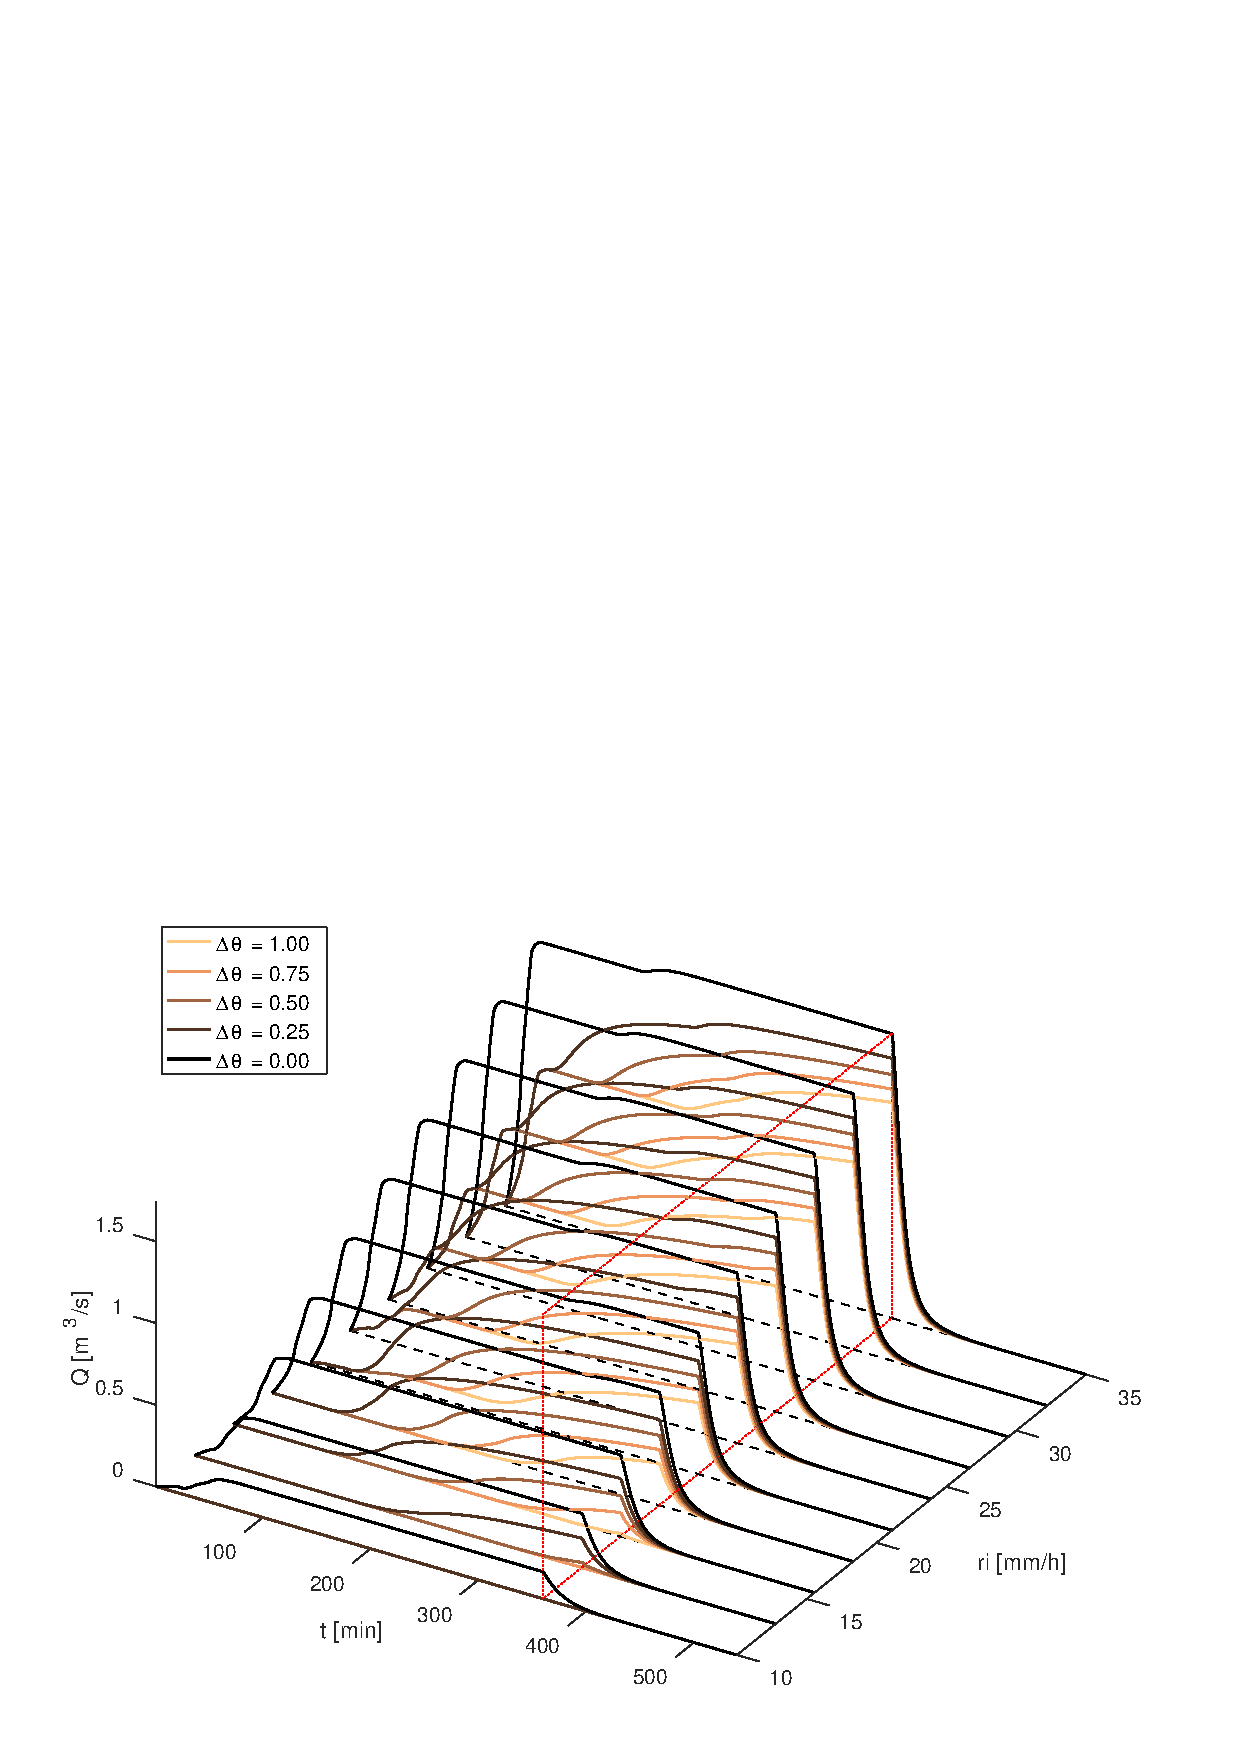
\includegraphics[width=0.8\textwidth]{img/hydrographs3d.png}
  \end{frame}
% * Here we can see the results extracted from the simulations. The plot shows the
%   different hydrographs at the channel outlet generated by the 50 different simulations.
% * The x-axis shows the time and z-axis the discharge. The y-axis corresponds 
%   to rain intensity. The initial soil saturation theta_i is indicated by the
%   different color tones. The red frame indicates the end of the rain events. From there
%   all hydrographs start to recess.
% * We can notice that some rain events produced absolutely no channel discharge.
% * Those with high initial soil saturation reached their peak discharge very fast.
% * Many hydrographs show an interesting behavior: a first plateau after some time,
%   where it seems that discharge won't grow any more, followed by one or two bumpy 
%   increases. These bumps are given by the topography. Two droplets at the same distance
%   from the outlet don't necessary have the same travel time. Those coming from
%   the "Gaussian mountains" will travel faster due to the slope. Those bumps are then
%   given by the water from the "plain" which is arriving later.


%%%%%%%%%%%%%%%%%%%%%%%%%%%%%%%%%%%%%%%%%%%%%%%%%%%%%%%%%%%%%%%%%%%%%%%%%%%%%%%%
% CASE STUDY 2: EXTRACT EMULATOR DATASET
  \begin{frame}
    \frametitle{Emulator dataset extraction}
    \centering
    \includegraphics[width=0.8\textwidth]{img/hydrograph.png}
  \end{frame}
% * The emulator we want to build should estimate the time needed by a given
%   rain event to generate the channel threshold discharge.
% * For this a threshold has to be chosen.
% * Here we can see, that depending on the threshold value Q! that we select,
%   the time-to-threshold t! can vary enormously: in the hydrograph raising limb
%   region fair variations of Q-threshold have almost no effect.
% * In the plateau region shown here by the two black lines the opposite is true:
%   a very small variation of the threshold value causes huge sudden variations 
%   of the time-to-threshold.
% * We conclude that the time-to-threshold is a very discontinuous quantity,
%   which is therefore very challenging to emulate.


%%%%%%%%%%%%%%%%%%%%%%%%%%%%%%%%%%%%%%%%%%%%%%%%%%%%%%%%%%%%%%%%%%%%%%%%%%%%%%%%
% CASE STUDY 2: CLASSIFY THE RAIN EVENTS
  \begin{frame}
    \frametitle{Rain events classification}
    \centering
    \includegraphics[width=0.8\textwidth]{img/classification.png}
  \end{frame}
% * In order to simplify the emulation task we first built a classifier 


%%%%%%%%%%%%%%%%%%%%%%%%%%%%%%%%%%%%%%%%%%%%%%%%%%%%%%%%%%%%%%%%%%%%%%%%%%%%%%%%
% CASE STUDY 2: EMULATE THE TIME-TO-THRESHOLD
  \begin{frame}
    \frametitle{\emph{Time-to-threshold} emulator}
    \centering
    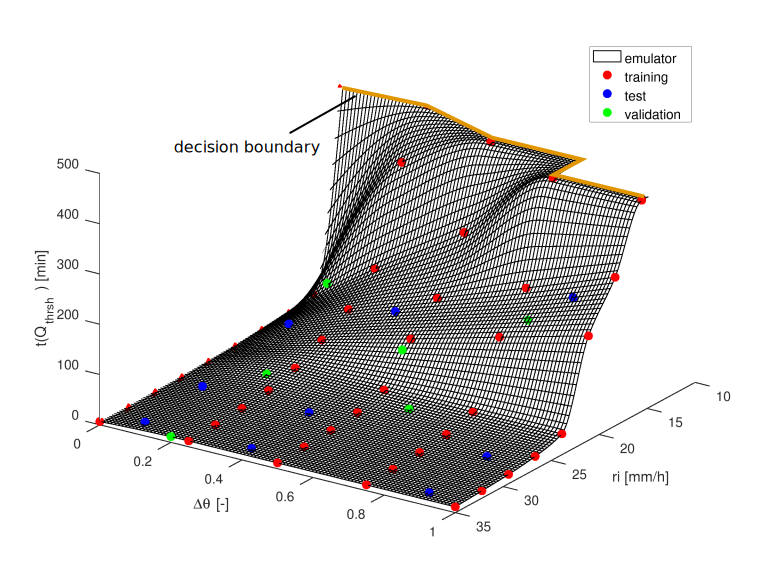
\includegraphics[width=0.8\textwidth]{img/emulator.png}
  \end{frame}


%%%%%%%%%%%%%%%%%%%%%%%%%%%%%%%%%%%%%%%%%%%%%%%%%%%%%%%%%%%%%%%%%%%%%%%%%%%%%%%%
% CONCLUSIONS
\section{Conclusion}

  \begin{frame}
    \frametitle{Conclusion}
    bla bla
  \end{frame}


%%%%%%%%%%%%%%%%%%%%%%%%%%%%%%%%%%%%%%%%%%%%%%%%%%%%%%%%%%%%%%%%%%%%%%%%%%%%%%%%
% OUTLOOK
\section{Outlook}

  \begin{frame}
    \frametitle{Outlook}
    bla bla
  \end{frame}


%%%%%%%%%%%%%%%%%%%%%%%%%%%%%%%%%%%%%%%%%%%%%%%%%%%%%%%%%%%%%%%%%%%%%%%%%%%%%%%%
% THE END
  {
  \setbeamertemplate{background}{}
  \setbeamercolor{background canvas}{bg=black}
  \setbeamercolor{normal text}{fg=white}
  \usebeamercolor[fg]{normal text}
  \begin{frame}[plain]
    \centering
    \Large{\textbf{THE END}}\\
  \end{frame}
  }



%:::::::::::::::::::::::::::::::::::::::::::::::::::::::::::::::::::::::::::::::
% * The whole procedure to develop this emulator with a real topography would have been
%   exactly the same, with the only difference that the simulations necessary to build
%   the emulator would have taken much longer.
%:::::::::::::::::::::::::::::::::::::::::::::::::::::::::::::::::::::::::::::::




%%%%%%%%%%%%%%%%%%%%%%%%%%%%%%%%%%%%%%%%%%%%%%%%%%%%%%%%%%%%%%%%%%%%%%%%%%%%%%%%
%%%%%%%%%%%%%%%%%%%%%%%%%%%%%%%%%%%%%%%%%%%%%%%%%%%%%%%%%%%%%%%%%%%%%%%%%%%%%%%%
% ADDITIONAL SLIDES
% Links to repositories
\section{Backup slides}
  \begin{frame}
    \frametitle{Links to my repositories}
    \small{\url{https://bitbucket.org/binello7/fswof2d}}\\
    \small{\url{https://bitbucket.org/binello7/master_thesis}}\\
    \small{\url{https://bitbucket.org/binello7/master_thesis/wiki/Home}}
  \end{frame}

% ------------------------------------------------------------------------------
% Case study 1: grid convergence study




\end{document}

